% Main paper. Needs macros.tex.
\begin{figure*}[t]
\centering
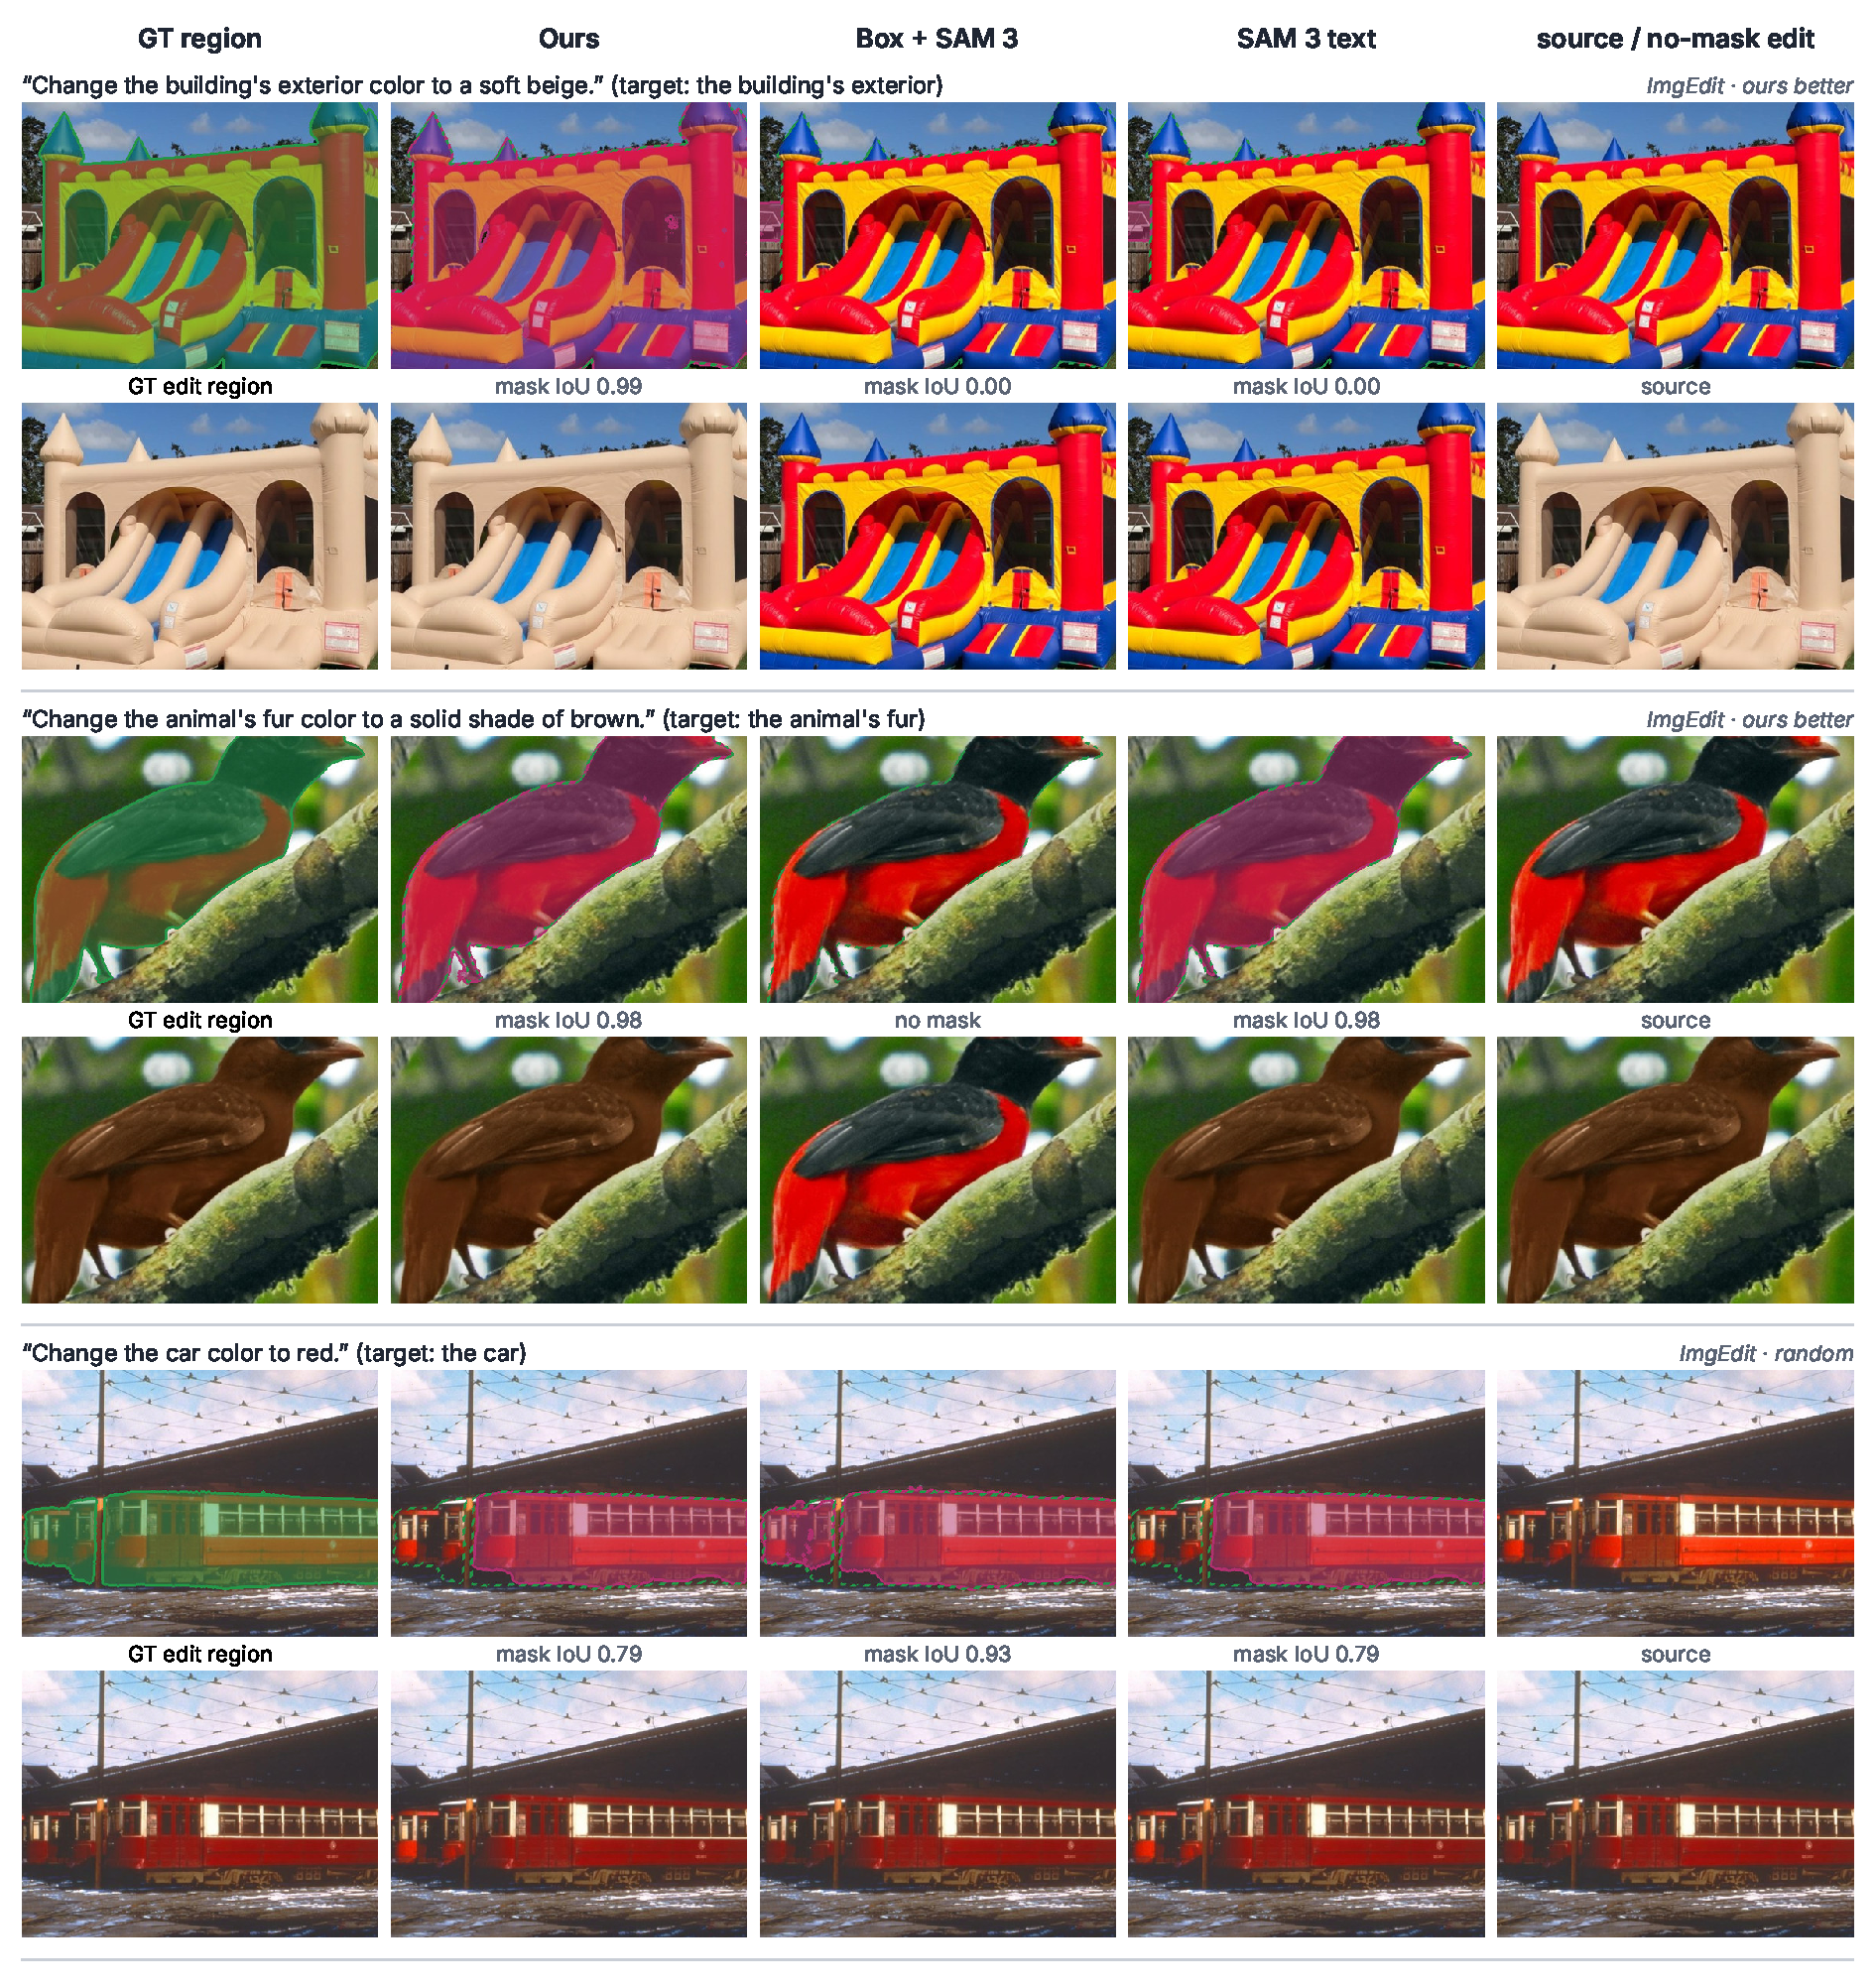
\includegraphics[width=\textwidth]{figures/qualitative/edit_main.pdf}
\caption{\textbf{Region-grounded editing} (ImgEdit-Bench, Qwen-Image-Edit; protocol of Tab.~\ref{tab:editing}). Top of
each sample: the mask each source localizes for the edit's referent (GT edit region dashed); bottom: the edit applied
within that mask, and the unmasked edit. A wrong or missing mask leaves the target unedited (rows 1--2: Box + SAM\,3
and SAM\,3 miss the building, Box + SAM\,3 returns no mask for the bird); row 3 is a random sample.}
\label{fig:qual_editing}
\end{figure*}
